% Fig. 4: Scheme comparison by source of guidance and training arrangement.
\begin{figure}[t]
\centering
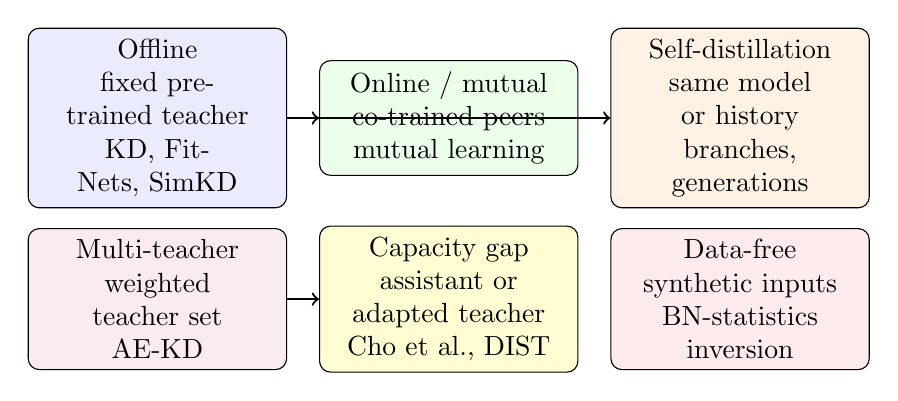
\begin{tikzpicture}[box/.style={draw,rounded corners,align=center,text width=3.0cm,minimum height=1.45cm,inner sep=4pt}, arr/.style={->,thick}]
\node[box,fill=blue!8] (offline) at (0,0) {Offline\\fixed pretrained teacher\\KD, FitNets, SimKD};
\node[box,fill=green!8] (online) at (3.7,0) {Online / mutual\\co-trained peers\\mutual learning};
\node[box,fill=orange!10] (self) at (7.4,0) {Self-distillation\\same model or history\\branches, generations};
\node[box,fill=purple!8] (multi) at (0,-2.3) {Multi-teacher\\weighted teacher set\\AE-KD};
\node[box,fill=yellow!18] (gap) at (3.7,-2.3) {Capacity gap\\assistant or adapted teacher\\Cho et al., DIST};
\node[box,fill=red!8] (free) at (7.4,-2.3) {Data-free\\synthetic inputs\\BN-statistics inversion};
\draw[arr] (offline) -- (online);
\draw[arr] (offline) -- (self);
\draw[arr] (multi) -- (gap);
\end{tikzpicture}
\caption{Training schemes differ in teacher availability, number of guidance sources, and whether original training data are available. Arrows indicate alternative arrangements, not a required progression.}
\label{fig:schemes}
\end{figure}
